\documentclass[10pt,conference]{IEEEtran}
\IEEEoverridecommandlockouts
% The preceding line is only needed to identify funding in the first footnote. If that is unneeded, please comment it out.
\usepackage{cite}
\usepackage{amsmath,amssymb,amsfonts}
\usepackage{algorithmic}
\usepackage{graphicx}
\usepackage{textcomp}
\usepackage{xcolor}
\usepackage{subfig}
\usepackage{listings}
\lstset{numbers=left,stepnumber=1,basicstyle=\footnotesize\ttfamily}
\def\BibTeX{{\rm B\kern-.05em{\sc i\kern-.025em b}\kern-.08em
    T\kern-.1667em\lower.7ex\hbox{E}\kern-.125emX}}
    \def\code#1{\texttt{#1}}
\begin{document}

\title{A Second Look at the Dynamics of the JavaScript Package Ecosystem\\}

\author{\IEEEauthorblockN{Kevin de Haan, Gregory Neagu, Frederic Sauve-Hoover, Abram Hindle}
\IEEEauthorblockA{\textit{Department of Computing Science} \\
\textit{University of Alberta}\\
Edmonton, Canada\\
Email: \{kdehaan,neagu,rsauveho,abram.hindle\}@ualberta.ca}
}

\maketitle

% Footnote should maybe be a full source, or just one link
\begin{abstract}
In recent years, the tools and packages most commonly involved with JavaScript development have evolved rapidly.
Newer packages such as Angular and React have experienced a marked increase in popularity among developers, while frameworks such as jQuery
have begun to phase out.\footnote{\label{adoption}https://insights.stackoverflow.com/survey/2016\#technology-most-popular-technologies, 
https://insights.stackoverflow.com/survey/2017\#technology-\_-frameworks-libraries-and-other-technologies, 
https://insights.stackoverflow.com/survey/2018\#technology-\_-frameworks-libraries-and-tools}
For this reason we take a second look at a 2016 paper by Wittern, Suter and Rajagopalan \cite{Wittern:2016} 
to see what aspects of the JavaScript package ecosystem have changed, and if previously observed trends have remained constant.
In the original paper the authors use the \emph{node package manager} (\code{npm}) to gain 
insight into the JavaScript ecosystem as a whole, and data from projects publicly hosted on 
\code{GitHub} to observe an alternative measure of popularity. We adhere to the same methods of analysis, 
and extend the data to capture more recent information up to April 1\textsuperscript{st} 2019.
Ultimately, this second look aims to discover if recent years have had any significant effects on 
ecosystem-wide trends, and provide developers with further insight into how packages are used and evolve.
\end{abstract}


\begin{IEEEkeywords}
JavaScript; Node.js; node package manager; software ecosystem analysis
\end{IEEEkeywords}


\section{Introduction}
Software ecosystems are environments that form as projects develop in parallel,
becoming interconnected as contexts and dependencies span companies and communities \cite{LUNGU2010264}. 
Research on these systems has increased rapidly in the recent past \cite{Manikas:2017}, investigating
their characteristics and behaviour as they develop \cite{Manikas:2013}. Understanding how software
ecosystems evolve is important from both a software as well as a business standpoint\cite{Messerschmitt},
and is valuable for informing developers how technologies are used over time \cite{Serebrenik:2015}. 
An understanding of software ecosystems can inform decisions on when to adopt frameworks and how long
to support them, as well as provide insight into how changes to software propagate throughout the community \cite{Wittern:2016}.
Additionally, determining the characteristics of software ecosystems 
can help clarify why some frameworks flourish while others fail, and guide 
developers in the creation of new tools\cite{Serebrenik:2015}. Furthermore, 
because software projects are overwhelmingly a collaborative effort, a complete
understanding of a single project often requires knowledge of the ecosystem supporting it\cite{Blincoe:2015}.


This paper is a replication of \emph{A Look at the Dynamics of the JavaScript Package Ecosystem}\cite{Wittern:2016} 
that performs extensive analysis of the \emph{node package manager} (\code{npm}) ecosystem. 
\code{npm} provides a set of open source tools that allow developers to 
describe packages for \code{Node.js}, an asynchronous JavaScript runtime environment 
designed for network applications\footnote{https://nodejs.org/en/about/}.
The services provided by \code{npm} include a command line interface for maintaining 
\code{package.json} files, the primary method to describe package metadata such as the name,
description, version, and dependencies of a given package. \code{npm} also allows 
developers to publish their packages to a public registry, permitting anyone 
to download and use their software. Packages hosted on \code{npm} will often depend on other \code{npm}
packages, forming an elaborate JavaScript package ecosystem.
Since the publishing of the original paper, the usage and scale of \code{npm} has only grown,
 and now hosts more than three times as many packages (over 750,000 as of April 1\textsuperscript{st} 2019) 
and handles over ten times as many weekly package downloads (now over ten billion per week).
Additionally, the major frameworks used in JavaScript development have undergone a 
rapid transformation as packages such as Angular and React are adopted\footnotemark[\ref{adoption}].
The core contributions we make are as follows:
\begin{itemize}
  \item We replicate and verify the results found in the original paper for the 
  window of October 1\textsuperscript{st} 2010 to September 1\textsuperscript{st} 2015.
  \item We extend the analysis to the time period of September 2\textsuperscript{nd} 
  2015 to April 1\textsuperscript{st} 2019, and evaluate whether patterns and trends 
  noted in the original paper are still observable.
  \item We investigate whether the continued evolution of the JavaScript package 
  ecosystem has affected the relationships between various measures of package popularity.
  \item We determine if the ongoing maturation of the \code{npm} ecosystem has 
  resulted in tangible changes to version numbering or adoption practices.
\end{itemize}




\section{Data Collection}
% CHECK IF THE NUMBERS ARE RIGHT
The window of data analyzed within this paper is October 1\textsuperscript{st} 2010 (as in the original paper) to April 1\textsuperscript{st} 2019.
We collected from three publicly available data sets. Two of these, the \code{npm} registry and the \code{GitHub} repository platform, are from the same source as in the original paper.
To find repositories relying on \code{npm}, we used the Google BigQuery \code{github\_repos} data set, updated weekly\footnote{https://github.com/fhoffa/analyzing\_github/}.
By using this set we are able to analyze \code{GitHub} data without being constrained to the currently available window provided by the GHTorrent project\cite{Gousi13}.
The final data set encompasses 797,940 packages and \textbf{\#VALUE} applications.

\subsection{Package Metadata}

\begin{lstlisting}[caption={A mock \code{npm} package.json. Some fields omitted for brevity.},captionpos=b,
  label=samplePkg, frame=single, firstline=1]
{
  "name": "Lorem Ipsum",
  "version": "0.9.3",
  "maintainers": [
      {"name": "Dolor Sit",
      "email": "dolorsit@amet.org"}
  ],
  "repository": {
      "type": "git",
      "url": "https://github.com/lor/em"
  },
  "main" : "loremipsum.js",
  "keywords": ["Web", "REST"],
  "dependencies": {
      "Adipiscing": "~1.7.0",
      "Elit": "5.1.x"
  },
  "devDependencies": {
      "Sed": "0.9.0",
      "Do": ">=1.3.5 <4.0.0" 
  }
}
\end{lstlisting}


\textbf{this one is probably mostly for @Fred}

\subsection{Applications using \code{npm} Packages}

\textbf{@Greg I'm gonna need you to put something here}

\section{Ecosystem Evolution}

Created in 2009, \code{npm} has grown
rapidly in popularity and scope over the last ten years, and 
as of the original paper showed no signs of slowing down \cite{Wittern:2016}.
We investigate the state of the \code{npm} ecosystem
since September 1\textsuperscript{st} 2015, and look for any signs of deterioration in 
the health of the ecosystem. Periods of stagnating growth would suggest
that developer interest is waning, while steady activity would 
indicate that the ecosystem as a whole is healthy and will continue to
evolve. To search for these potential indicators in the \code{npm} package environment,
we investigate the number of packages created and updated over time, as well
as system-wide trends of dependencies within packages. In figure 1 
[INSERT DATA COMMENTARY HERE]. Figure 2 [MORE DATA COMMENTARY].

To better visualize the status of inter-package dependencies, we constructed
a directed dependency graph using dependants as out-degrees and
dependencies as in-degrees. Based on this dependency graph, Figure \ref{outDegree}
displays the percentage of packages with various amounts of dependencies. 
[MIGHT NEED TO CHANGE BASED ON DATA: While the average number of dependencies 
of packages continues to increase, the percentage of packages with zero 
to three dependencies has actually increased since the end of the original paper's
reporting period \cite{Wittern:2016}. This suggests some changes to developer 
behaviour, likely either as a deliberate effort by programmers seeking to avoid the perils of 
complicated dependency trees \cite{Kikas:2017}, or as a natural result of the ever-changing
ways in which JavaScript is used for project development. [ADD EXACT VALUES]

\begin{figure}
  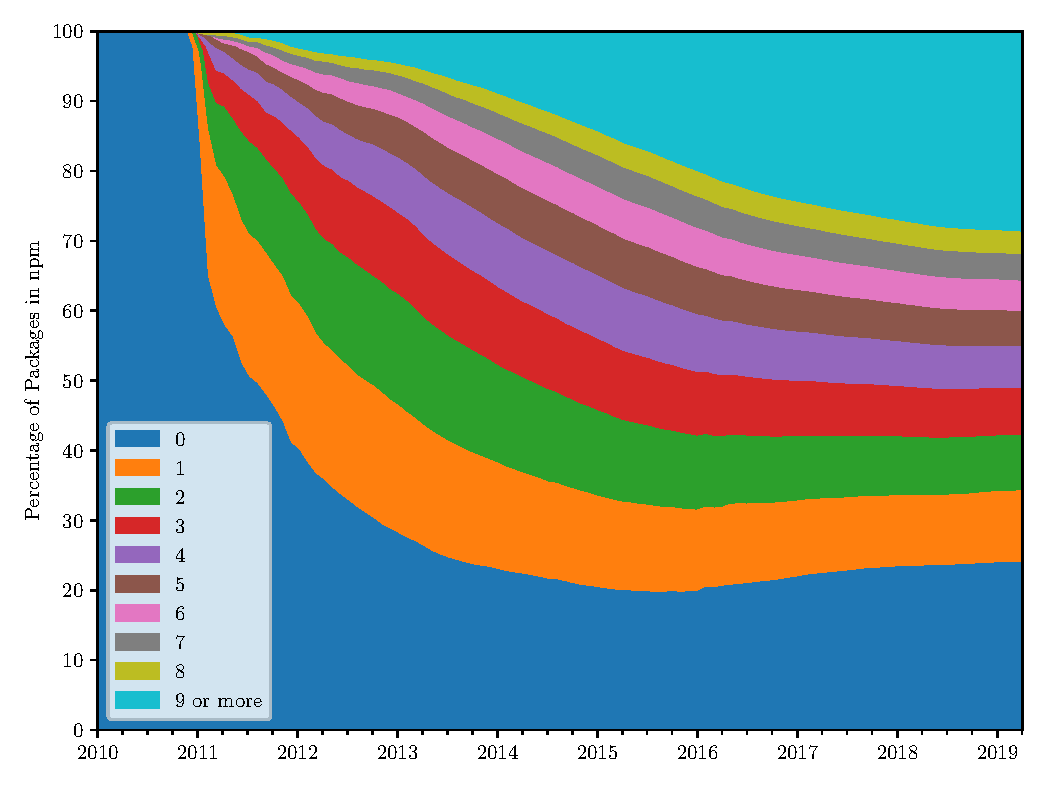
\includegraphics[width=0.5\textwidth]{figures/npm_deps_monthly_out_degree.pdf}
  \caption{\code{npm} packages by their number of dependencies on other packages}
  \label{outDegree}
\end{figure}

\begin{figure}
  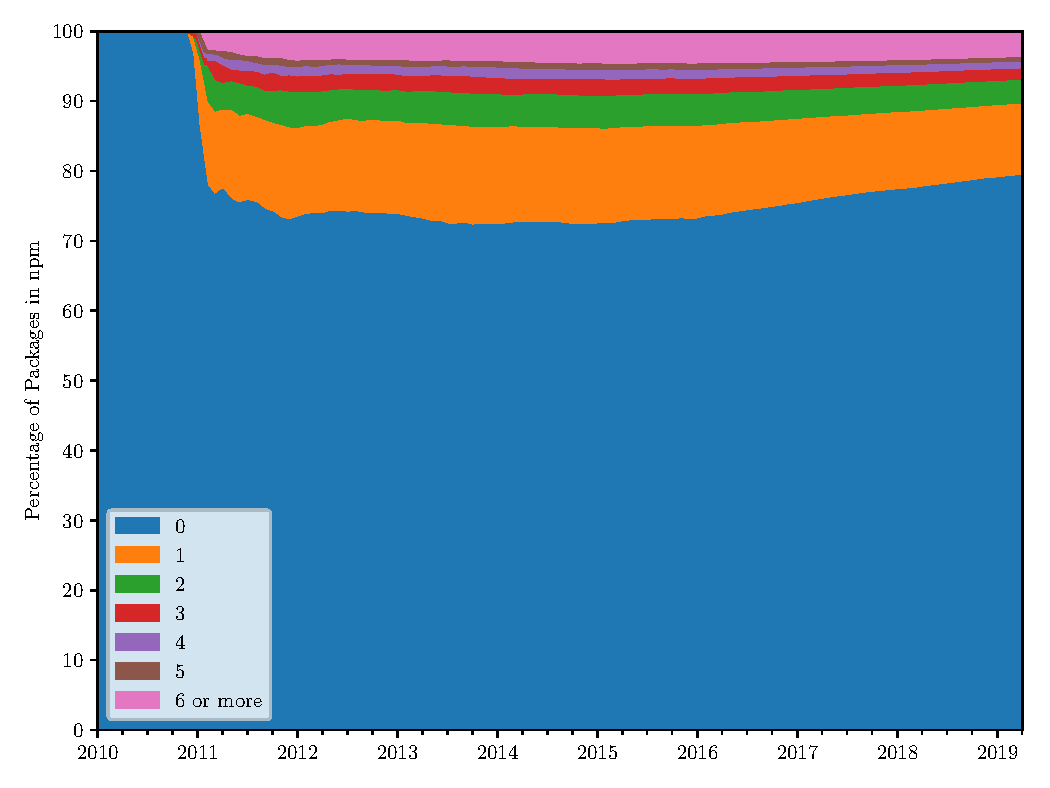
\includegraphics[width=0.5\textwidth]{figures/npm_deps_monthly_in_degree.pdf}
  \caption{\code{npm} packages by the number of other packages depending on them}
  \label{inDegree}
\end{figure}




\section{Package Popularity}



\subsection{Relationships between Measures}

\subsection{Distinct Package Types}

\subsection{Popularity Over Time}


\subsubsection{Identifying Top Packages}

\subsubsection{Popular Package Dynamics}

\begin{figure*}
  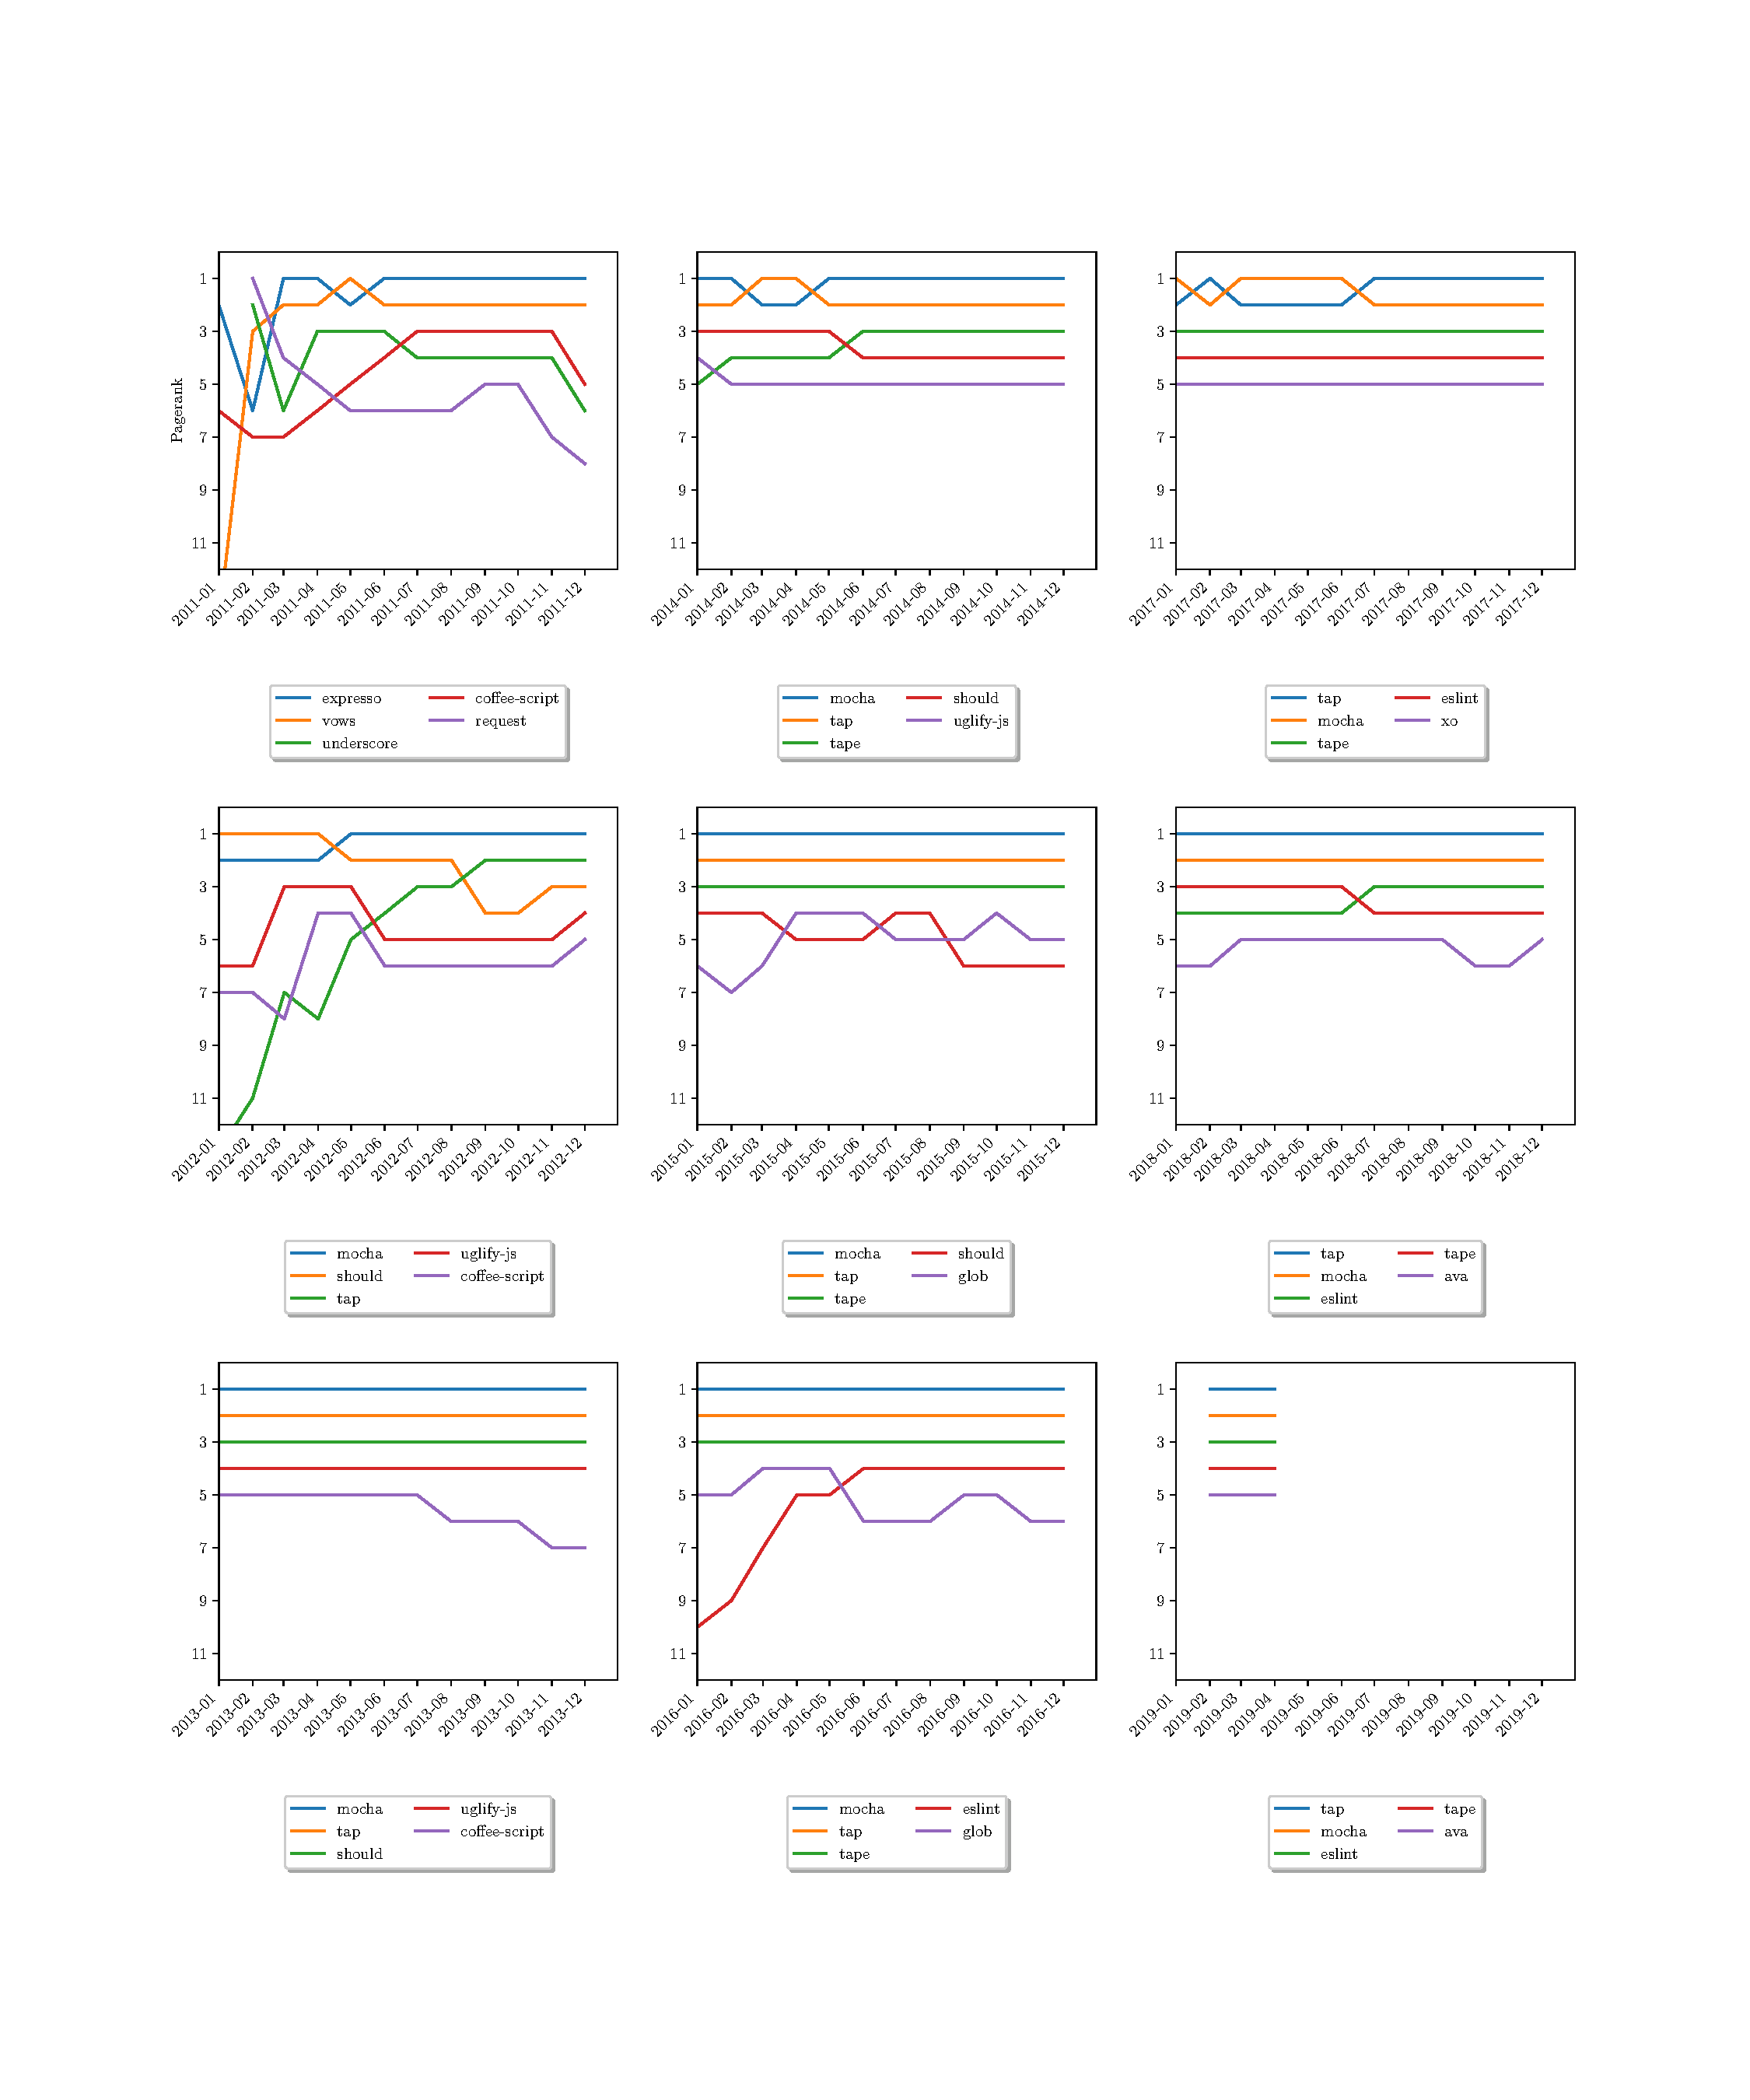
\includegraphics[width=1\textwidth]{figures/highest_ranked.pdf}
  \caption{\code{npm} rank (based on pagerank) of five packages with the lowest geometric mean per year}
  \label{ranksByYear}
\end{figure*}

\begin{figure}
  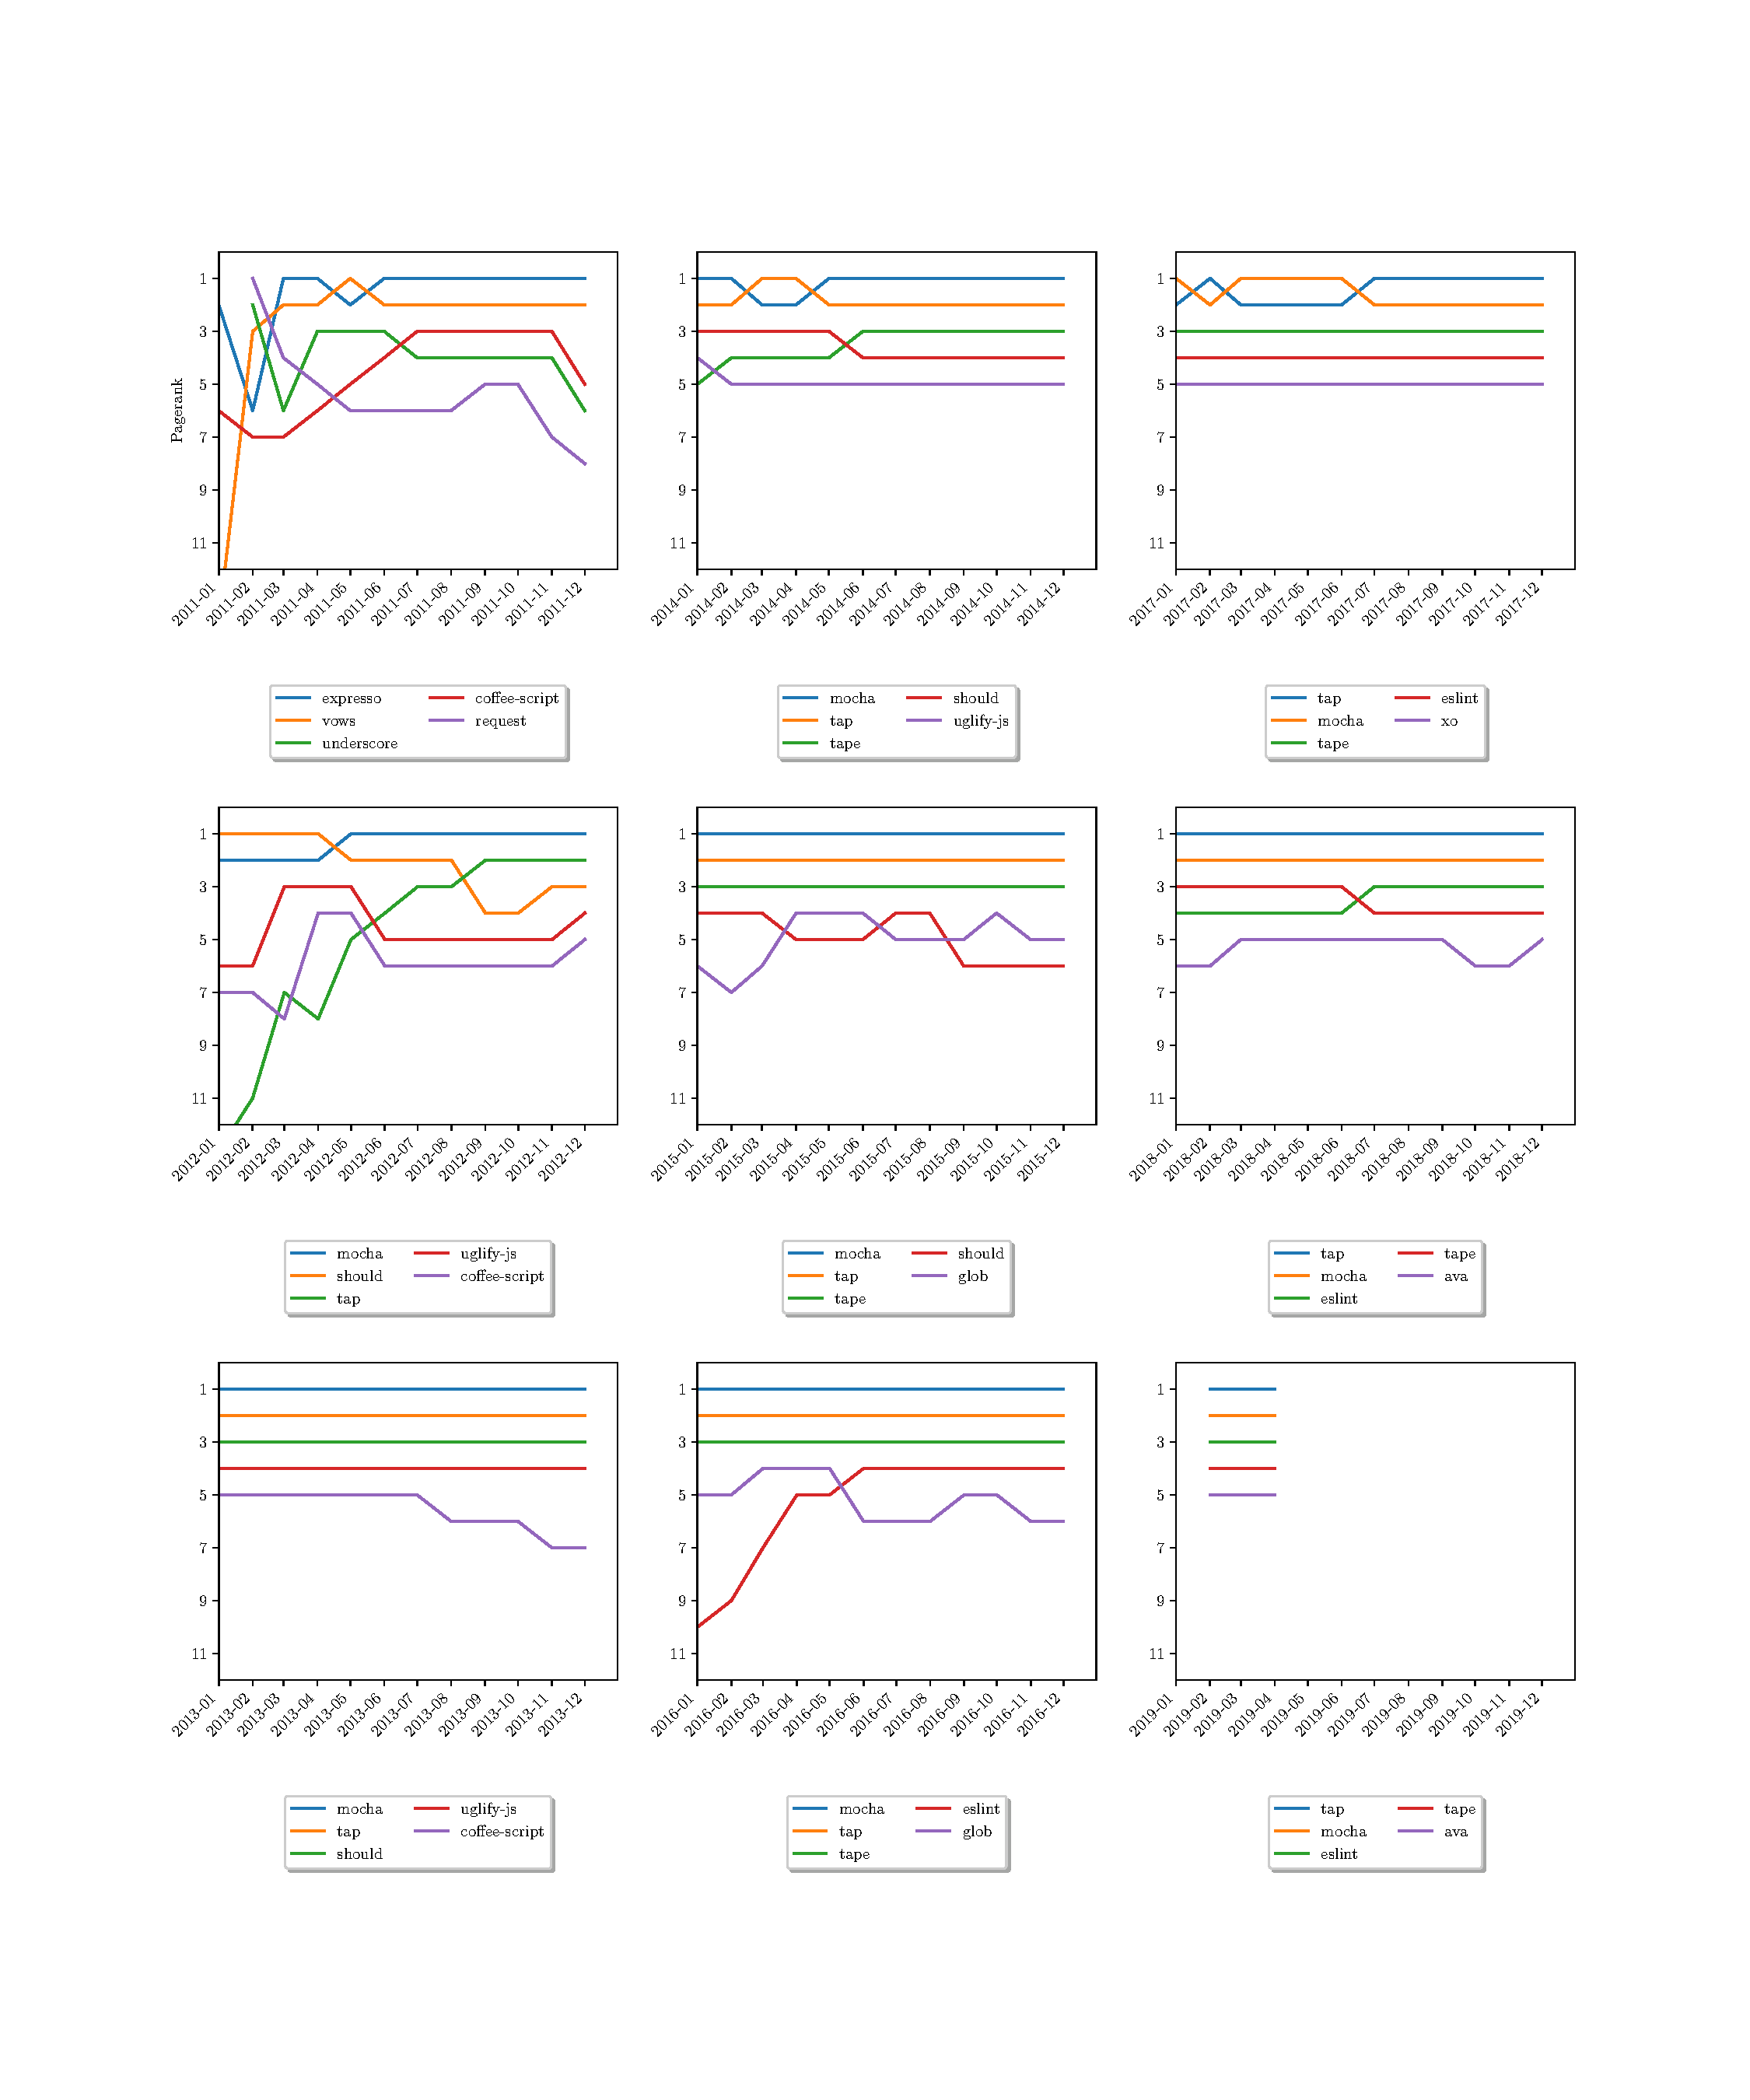
\includegraphics[width=0.5\textwidth]{figures/highest_ranked.pdf}
  \caption{\code{npm} rank (based on pagerank) of five packages with the lowest geometric mean per year}
  \label{ranksByYear}
\end{figure*}

\subsubsection{Comparing Popularities}

\section{Version Numbering and Package Adoption}

\subsection{Attribution of Version Numbers}

\subsection{Adoption by Version Number}

\section{Related Work}

\section{Conclusion}


\begin{thebibliography}{00}

  \bibitem{Blincoe:2015}
  Kelly Blincoe, Francis Harrison, and Daniela Damian.
  \newblock Ecosystems in github and a method for ecosystem identification using
    reference coupling.
  \newblock In {\em Proceedings of the 12th Working Conference on Mining Software
    Repositories}, MSR '15, pages 202--207, Piscataway, NJ, USA, 2015. IEEE
    Press.
  
  \bibitem{DBLP:Decan:2018}
  Alexandre Decan, Tom Mens, and Philippe Grosjean.
  \newblock An empirical comparison of dependency network evolution in seven
    software packaging ecosystems.
  \newblock {\em CoRR}, abs/1710.04936, 2017.
  
  \bibitem{Gousi13}
  Georgios Gousios.
  \newblock The ghtorrent dataset and tool suite.
  \newblock In {\em Proceedings of the 10th Working Conference on Mining Software
    Repositories}, MSR '13, pages 233--236, Piscataway, NJ, USA, 2013. IEEE
    Press.
  
  \bibitem{Kikas:2017}
  Riivo Kikas, Georgios Gousios, Marlon Dumas, and Dietmar Pfahl.
  \newblock Structure and evolution of package dependency networks.
  \newblock In {\em Proceedings of the 14th International Conference on Mining
    Software Repositories}, MSR '17, pages 102--112, Piscataway, NJ, USA, 2017.
    IEEE Press.
  
  \bibitem{LUNGU2010264}
  Mircea Lungu, Michele Lanza, Tudor Gîrba, and Romain Robbes.
  \newblock The small project observatory: Visualizing software ecosystems.
  \newblock {\em Science of Computer Programming}, 75(4):264 -- 275, 2010.
  \newblock Experimental Software and Toolkits (EST 3): A special issue of the
    Workshop on Academic Software Development Tools and Techniques (WASDeTT
    2008).
  
  \bibitem{Manikas:2013}
  Konstantinos Manikas and Klaus~Marius Hansen.
  \newblock Software ecosystems - a systematic literature review.
  \newblock {\em J. Syst. Softw.}, 86(5):1294--1306, May 2013.
  
  \bibitem{Messerschmitt}
  David Messerschmitt and Clemens Szyperski.
  \newblock {\em Software Ecosystem: Understanding an Indispensable Technology
    and Industry}.
  \newblock 01 2003.
  
  \bibitem{DBLP:PanoGA16}
  Amantia Pano, Daniel Graziotin, and Pekka Abrahamsson.
  \newblock What leads developers towards the choice of a javascript framework?
  \newblock {\em CoRR}, abs/1605.04303, 2016.
  
  \bibitem{Manikas:2017}
  M.~{Seppänen}, S.~{Hyrynsalmi}, K.~{Manikas}, and A.~{Suominen}.
  \newblock Yet another ecosystem literature review: 10+1 research communities.
  \newblock In {\em 2017 IEEE European Technology and Engineering Management
    Summit (E-TEMS)}, pages 1--8, Oct 2017.
  
  \bibitem{Serebrenik:2015}
  Alexander Serebrenik and Tom Mens.
  \newblock Challenges in software ecosystems research.
  \newblock In {\em Proceedings of the 2015 European Conference on Software
    Architecture Workshops}, ECSAW '15, pages 40:1--40:6, New York, NY, USA,
    2015. ACM.
  
  \bibitem{Wittern:2016}
  Erik Wittern, Philippe Suter, and Shriram Rajagopalan.
  \newblock A look at the dynamics of the javascript package ecosystem.
  \newblock In {\em Proceedings of the 13th International Conference on Mining
    Software Repositories}, MSR '16, pages 351--361, New York, NY, USA, 2016.
    ACM.
  
  \end{thebibliography}
  
\vspace{12pt}

\end{document}
